\chapter{DESENVOLVIMENTO}
O desenvolvimento deve conter a fundamentação teórica, a metodologia e a análise e discussão dos resultados, que podem ser apresentados em forma de tabelas ou gráficos. Pode ser dividido em seções e subseções conforme a função da abordagem do tema.

\section{Fundamentação Teórica}
Nesta seção é apresentado um debate acerca do que os pesquisadores falam acerca do tema escolhido para a pesquisa. Privilegie o máximo de fontes diferentes (artigos, teses, dissertações, monografias e livros). Exemplo de citação \cite{towfic2022benchmarking}.

Segundo \citeonline{chu2021sustained}, isto é um outro exemplo de citação.

\begin{citacao}
Injeção de dependências (\textit{dependency injection} ou DI) é um padrão de
desenvolvimento de software usado para manter o baixo acoplamento entre classes do
sistema. As dependências de um objeto não são instanciadas programaticamente, mas
sim injetadas de alguma forma \cite{chambers2021macbook}.
\end{citacao}

\section{Metodologia}
Nesta seção é apresentado o método e delimitada a metodologia (quanto à abordagem: quantitativa ou qualitativa; quanto aos objetivos: explicativa, descritiva ou exploratória; e, quanto aos procedimentos).

\begin{figure}[htb]
    \centering
	\caption{\label{fig:bpmn-modelagem}Representação da estrutura do Spring Data}
	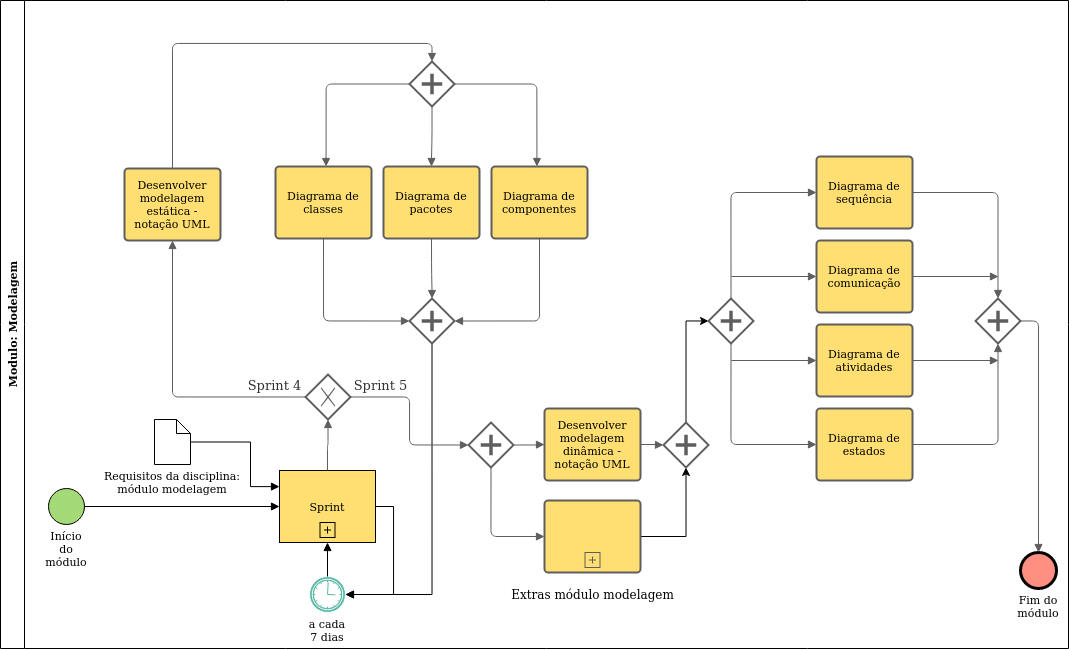
\includegraphics[width=0.85\linewidth]{img/bpmn_modelagem.png}
	\fonte{\citeonline{ribeiro2015beneficios}}
\end{figure}

\section{Análise e Discussão dos Resultados}
Nesta seção são apresentados e discutidos os resultados obtidos. Este é o exemplo de uso de notas de rodapé. O sistema foi desenvolvido utilizando a arquitetura de microsserviços\footnote{Para mais informações acesse: \url{https://aws.amazon.com/pt/microservices/}} para garantir maior escalabilidade.

\begin{table}[htb]
\centering
\caption{Exemplo de tabela de resultados}
\begin{tabular}{|l|c|c|c|}
\hline
\textbf{Item} & \textbf{Métrica A} & \textbf{Métrica B} & \textbf{Métrica C} \\ \hline
Resultado 1 & X & X & X \\ \hline
Resultado 2 & X & X & X \\ \hline
Resultado 3 & X & X & X \\ \hline
\end{tabular}
\fonte{Elaborado pelo autor (\the\year).}
\end{table}
